% Copyright 2004 by Till Tantau <tantau@users.sourceforge.net>.
%
% In principle, this file can be redistributed and/or modified under
% the terms of the GNU Public License, version 2.
%
% However, this file is supposed to be a template to be modified
% for your own needs. For this reason, if you use this file as a
% template and not specifically distribute it as part of a another
% package/program, I grant the extra permission to freely copy and
% modify this file as you see fit and even to delete this copyright
% notice. 


\documentclass[9pt]{beamer}
\usepackage{graphicx}                       % loads images
\usepackage{color}                          % for color in text
\usepackage{float}                          % to place [H]
\usepackage{amsmath}
\usepackage{amssymb}
\usepackage{bbm}
\usepackage{booktabs}
\usepackage{longtable}
\usepackage{bigstrut}
\usepackage{array}

    
\usepackage{tikz}
\usetikzlibrary{shapes.geometric, arrows}
\usepackage{multirow}
\usepackage{xr}
%\usepackage[round]{natbib}



\usepackage[backend=biber, style=alphabetic ,
citestyle=authoryear]{biblatex}
  % biber is version 2.4; the latest?


\addbibresource{../paper/References.bib}




\graphicspath{{../paper/Figuras/}}
\usepackage{color}
%\usepackage{morefloats}
%\usepackage{showkeys}

\usepackage{enumerate}
\usepackage[labelfont=bf]{caption}
\usepackage[labelfont=bf, justification=justified]{subcaption}
\captionsetup{position=top}
\captionsetup[subfigure]{justification=centering}



\usepackage{epstopdf}
\epstopdfDeclareGraphicsRule{.tiff}{png}{.png}{convert #1 \OutputFile}
\AppendGraphicsExtensions{.tiff}


\usepackage{setspace}

\renewcommand{\rmdefault}{ppl}
\definecolor{darkred}{rgb}{0.8, 0.0, 0.0}
\definecolor{navyblue}{rgb}{0.0, 0.0, 0.8}
\definecolor{cadmiumgreen}{rgb}{0.0, 0.6, 0.24}

\usepackage{hyperref}
\hypersetup{
    pdfstartview={FitH},    		% fits the width of the page to the window
    pdftitle={Statistical information and settlement: evidence from Mexican Labour courts},    % title
    pdfauthor={IML},     % author
    colorlinks=true,       % false: boxed links; true: colored links
    linkcolor=black,          % color of internal links (change box color with linkbordercolor)
    citecolor=darkred,        % color of links to bibliography
    filecolor=magenta,      % color of file links
    urlcolor=darkred           % color of external links
}

\newcommand{\green}[1]{\textcolor{cadmiumgreen}{#1}}

\newcommand{\comment}[1]
{\par {\bfseries \color{blue} #1 \par}}
%\usepackage{showkeys}
\setbeamertemplate{theorems}[numbered]
\newtheorem{theorem}{}
\newtheorem{claim}[theorem]{Claim}


% There are many different themes available for Beamer. A comprehensive
% list with examples is given here:
% http://deic.uab.es/~iblanes/beamer_gallery/index_by_theme.html
% You can uncomment the themes below if you would like to use a different
% one:
%\usetheme{AnnArbor}
%\usetheme{Antibes}
%\usetheme{Bergen}
%\usetheme{Berkeley}
%\usetheme{Berlin}
%\usetheme{Boadilla}
%\usetheme{boxes}
%\usetheme{CambridgeUS}
%\usetheme{Copenhagen}
%\usetheme{Darmstadt}
%\usetheme{default}
%\usetheme{Frankfurt}
%\usetheme{Goettingen}
%\usetheme{Hannover}
%\usetheme{Ilmenau}
%\usetheme{JuanLesPins}
%\usetheme{Luebeck}
\usetheme{Madrid}
%\usetheme{Malmoe}
%\usetheme{Marburg}
%\usetheme{Montpellier}
%\usetheme{PaloAlto}
%\usetheme{Pittsburgh}
%\usetheme{Rochester}
%\usetheme{Singapore}
%\usetheme{Szeged}
%\usetheme{Warsaw}

\setbeamertemplate{headline}{%
    \leavevmode%
    \hbox{%
        \begin{beamercolorbox}[wd=\paperwidth,ht=2.5ex,dp=1.125ex]{palette quaternary}%
            \insertsectionnavigationhorizontal{\paperwidth}{}{\hskip0pt plus1filll}
        \end{beamercolorbox}%
    }
}

\title{Information and Bargaining through Agents: }

% A subtitle is optional and this may be deleted
\subtitle{Experimental Evidence from Mexico's Labor Courts}

\author{J. Sadka\inst{1} \and E. Seira\inst{2} \and C. Woodruff\inst{3}}
% - Give the names in the same order as the appear in the paper.
% - Use the \inst{?} command only if the authors have different
%   affiliation.

\institute[ITAM, Oxford] % (optional, but mostly needed)
{
  \inst{1,2}%
  ITAM
  \and
  \inst{3}%
  Oxford
}
% - Use the \inst command only if there are several affiliations.
% - Keep it simple, no one is interested in your street address.

\date{April 2018}
% - Either use conference name or its abbreviation.
% - Not really informative to the audience, more for people (including
%   yourself) who are reading the slides online

\subject{Applied Microeconomics}
% This is only inserted into the PDF information catalog. Can be left
% out. 

% If you have a file called "university-logo-filename.xxx", where xxx
% is a graphic format that can be processed by latex or pdflatex,
% resp., then you can add a logo as follows:

% \pgfdeclareimage[height=0.5cm]{university-logo}{university-logo-filename}
% \logo{\pgfuseimage{university-logo}}

% Delete this, if you do not want the table of contents to pop up at
% the beginning of each subsection:

% Let's get started
\begin{document}

\begin{frame}
  \titlepage
\end{frame}





\section*{Outline}
\begin{frame}{Outline}
\tableofcontents
\end{frame}



\section{Motivation}

\begin{frame}{Motivation}{}
  \begin{itemize}
  \item {Courts function poorly in most developing countries: backlogs, delay, unpredictable case outcomes. This hampers the functioning of markets and raises concerns about access to justice.}
  \vspace{.1in}
  \item {Little evidence on the ineffectiveness of courts and its causes.}
  \vspace{.1in}
  \item{Recently Mexico passed a constitutional reform that creates a compulsory pre-lawsuit  conciliation stage}...still under design.
  \vspace{.1in}
    \begin{itemize}
       \item Can providing statistical information to parties increase settlement?
       \item Can ``forcing'' a conciliation encounter increase settlement?
       \vspace{.05in}
    \end{itemize}
    
    \vspace{.1in}
    \item {This presentation:}
       \begin{itemize}
           \item First document some \alert{stylized facts} about settlement and misinformation in a Mexican labor court.
           \item Then show the results of an \alert{experiment} aimed at increasing the information available to parties on ongoing cases, who then decide whether to settle or continue a lawsuit.
       \end{itemize}
  \end{itemize}
\end{frame}
                  
\section{Context: Bargaining and agency}

%\section{Bargaining}
\begin{frame}{Motivation: Bargaining}

Courts are a disciplining device for a bargaining game between the plaintiff and defendant. 
   \begin{itemize}
       \item Most cases reached a bargained settlement. 
       \item The 60\% settlement rate in Mexico is lower than rates of 70\% in Australia, 80\% in the U.S. 90\ in Sweden, etc.  
   \end{itemize}
   
  \end{frame}
  
  
\begin{frame}{Motivation: Bargaining}

Rubenstein's (1982) canonical bargaining model shows under certain conditions, bargaining is efficient and settlement is immediate. \pause
\\
\vspace{.1in}
Unfortunately, reality intervenes: Most real world bargaining situations are characterised by asymmetric information. 
\vspace{.1in}
\\
Myerson - Sattherthwaite (1983) shows that bargaining may be inefficient when the parties have asymmetric information. 
    \begin{itemize}
        \item Settlement may not be reached even when it is beneficial for both parties. [On this, also Cramton 1991, 1992, Cramton and Tracy 1994a, 1994b]
    \end{itemize}
\pause
In addition to information asymmetries, excess optimism by the parties may also lead to bargaining breakdown (e.g., Yildiz 2011)

  
\end{frame}

\begin{frame}{Agency and Bargaining}

The bargaining literature focuses on a game between two parties (\textit{so far as we have found}). 
\\
\vspace{.1in}
But there are four parties in court cases:
\begin{itemize}
    \item the plaintiff
    \item the plaintiff's lawyer
    \item the defendant
    \item the defendant's lawyer
\end{itemize}
\vspace{.2in}
\end{frame}


\begin{frame}{Agency and bargaining}
The addition of agents may have positive or negative effects.
\vspace{.2in}
\begin{itemize}
%\item Gilson and Mnookin (1994): If legal proceedings are a prisoner's dilemma, then lawyers may generate cooperation where the parties themselves cannot. 
\\
\vspace{.2in}

\item  lawyers may be like expert agents. Their incentives may not align perfectly with their clients, creating more standard agency concerns. \begin{itemize}
    \item A substantial literature on expert agents: Levitt and Syverson (2008); Emons (1997); Schneider (2012), etc.
\end{itemize}
\vspace{.2in}
Our experiments will suggest the agents-as-experts view is more relevant in the labour courts. 
\end{itemize}
 

\end{frame}

\begin{frame}{Motivation: Agency and Bargaining}{}

In a bargaining environment characterized by asymmetric information and agency, we conduct experiments to provide evidence on three questions: 
\begin{enumerate}
      \item Does providing information on expected outcomes increase settlement rates, either by reducing information asymmetries or by reducing overconfidence? 
      \item Is there evidence that agency issues are important in the bargaining process?
      \item Is the welfare of the parties, and the plaintiffs in particular, improved by the provision of information? 
  \end{enumerate}
  
 \end{frame}
 
%\begin{frame}{Related Literature}
%\begin{itemize}
%    \item Effects of courts: \cite{Botero_Regulation},  %\cite{PonticelliAlencar_Bankrupcy}, %\cite{Kondylis_Stein_Senegal}
%    \vspace{.1in}
%    \item Bargaining and delay in litigation. 
%        \begin{itemize}
%        \item Informational asymmetries: credibly communicate %private value through inefficient waiting %(\cite{Cramton_1991, Cramton_1992}, \cite{Cramton_1994a, %Cramton_1994b})
%        \item Overconfidence: (\cite{Yildiz_CommonPrior}, \cite{Farber_DivergentExpectations})
%        \item Behavioral biases: (\cite{BabcockLoewensein_BargainingImpasse}, \cite{camerer_behavioral}).
%    \end{itemize}
%    \vspace{.1in}
%    \item Experts with incentives to lie or hide information from clients:
%    \cite{emons},
%    \cite{domenighetti}.
%    \vspace{.1in}
    %\item Lab experiments with bargaining and litigation settings: \cite{Ashenfelter_DisputeRates}, \cite{Pogarsky_DamageCaps}, and  \cite{Sullivan_Experimental}.
%    \vspace{.1in}
%    \item We know of no field experiment conducted in labor courts studying the decision of parties to settle.
%\end{itemize}
%\end{frame}


\section{Context}

\begin{frame}{Context}
   \begin{itemize}

       \item \textbf{The lawsuits:} We deal with firing disputes, courts must determine fair/unfair dismissal. 
       \vspace{0.05in}
         
        \item \textbf{The law:} Proving fair dismissal is difficult; legal severance is a minimum of three months' wage with benefits.  
        \vspace{0.05in}
         
        \item \textbf{The court:} We work with the Mexico City Labor Court (MCLC).
        \vspace{0.05in}
        \begin{itemize}
            \item Largest local labor court in Latin America (receives 30,000 new cases per year).
            \item Its backlog would take 4 years to process.
        \end{itemize}
                                
       %\item \textbf{Conciliation mandated by law:} The first hearing is supposedly dedicated to "conciliation". The MCLC has 1 assigned conciliator per individual court.
       %\vspace{0.05in}
       
       \item \textbf{What happens if they don't settle:} Defendant answers, evidence is submitted and viewed, and the court issues a judgment.
       \vspace{0.05in}
       
       \item \textbf{Enforcement:} is not trivial: 40 percent of decisions favorable to the worker uncollectable. 
       
       \end{itemize}         
        
     \end{frame}
     
     
\begin{frame}{... More context}
    \begin{itemize}     
       \item \textbf{Lawyers:} Legal representation is necessary to file a lawsuit. Lawyers dominate the process of the lawsuit. The presence of the parties themselves at the hearings is not compulsory. 
       \vspace{0.05in}
       
        \item   \textbf{Workers:} can hire private lawyers or a free lawyer from the public labor prosecutor's office.
        \vspace{0.05in}
            \begin{itemize}
                \item Public lawyers:
                \begin{itemize}
                    \item Paid a flat wage and cannot charge additional fees.
                    \item Generally well qualified, but overworked: they handle 10 times more cases on average.
                \end{itemize}
                \vspace{0.05in}
                \item Private lawyers:
                \begin{itemize}
                    \item They must be licensed, but do not have to pass a bar exam.
                    \item Charges: initial fee to file the lawsuit (around 100 USD), contingency fee of 30-40 percent.
                    \item Large variation in quality (anecdotal evidence).
                     \item \textbf{Partner:} Mexico City Labor Court.
       \vspace{0.1in}
                \end{itemize} 
            \end{itemize}

    \end{itemize}
\end{frame}


\begin{frame}{Experimental Design}{}
\textbf{Interventions:} The experiment was conducted with parties in ongoing cases in two phases:
%\begin{itemize}
  %              \item Lawyers almost always present, worker present about 20\% of the time.
 %        \end{itemize}
   \begin{itemize}
       \item Phase I: 
       \begin{itemize}
           \item A single sub-court (7)
           \item 1103 cases, March - May 2016
           \item Interventions on information and conciliation
           \item hearings at all points of the process
           \item Casefile level randomization
       \end{itemize}
  \pause     
       \item Phase II: 
       \begin{itemize}
           \item Scale-up to an additional 4 sub-courts
           \item \~1300 cases, October 2016 - March 2017
           \item Information treatment only (+ placebo)
           \item First hearings only
           \item Day level randomization
       \end{itemize}
       \end{itemize}
\pause
       \item \textbf{Outcomes}
       \begin{itemize}
           \item We use administrative records of the court to trace case outcomes
           \item We conduct surveys before [and after] treatments to measure expectations (and other variables)
       \end{itemize}

\end{frame}

\begin{frame}{Design, Phase I}{}
   \begin{itemize}
   
        \item \textbf{Participants:} Randomly assign parties to cases with hearings on the day to one of three conditions:
        
        \begin{enumerate}
            \item Information from a``Calculator'' with a range of predicted outcomes based on the characteristics of their case (e.g., wage and tenure). 
            \item Requested parties to sit with the sub-court's conciliator before proceeding with the hearing
            \item A control condition with neither of these two.
        \end{enumerate}
   
                \vspace{0.05in}
    \item \textbf{Baseline survey}: education, how they found their lawyer, payment to lawyer, expectations about win probability and amount, lawsuit duration, knowledge of the law and of own claims, expectations.
                \vspace{0.05in}
    \item \textbf{Exit survey}: Expectations (only for those that did not settle) .
   \end{itemize}
\end{frame}






\begin{frame}{Why might we expect the treatments to work?}

    \begin{itemize}
        \item \textbf{Low information environment}: Suing workers have:
        \begin{itemize}
            \item Little information of the law
            \item No repeated experience
            \item Propensity to biased expectations (selection, angry)
        \end{itemize}
        \vspace{0.1in}
        \item \textbf{Incentives of Private Lawyers:} Inflating the claim and not settling. Why?
        \begin{itemize}
                \item Less risk averse than the worker as they handle many cases
                \item They make a profit from just filing 
                %\item Even bad lawyers have some low probability of winning, due to excessive formalism, the low quality of the labor courts, and corruption. ESTO LO QUITE PORQUE AQUI SI ESTA ALINEADO CON EL WORKER
         \end{itemize}
          \vspace{0.1in}
        \item Private lawyers have more information than workers and anecdotally convince worker to sue by inflating their expectations of winning. 
\vspace{0.1in}
        \item{Our findings are consistent with this story, and we propose an analytic framework that explains the results. But it is not easy to prove...} 
            \begin{itemize}
                \item The main problem is that lawyers selection is endogenous to claims, misinformation, and unobservable case quality.
            \end{itemize}
    \end{itemize}
\end{frame}








\section{Data}

\begin{frame}{Data}{}
   \begin{itemize}

        \item \textbf{Historical Data:} Use it for diagnostics and \alert{``Calculator prediction''}.
        \vspace{0.05in}
            \begin{itemize}
                \item \textbf{Sample:} 2500 \textit{concluded} cases from subcourt 7 / 5000 \textit{concluded} cases from 5 subcourts. Random sample of all cases filed in 2011  which were concluded by the end of 2015.
                \vspace{0.05in}
                    
                \item \textbf{Variables:} Initial labor suit variables (e.g. wage, tenure); When the suit ended and how (settlement, drop, judgment, or expiry); compensation received by the worker.
            \end{itemize}
            \vspace{0.1in}
        \item \textbf{Survey data:} 70\% of cases with notified hearings conducted between March and May 2016: 1103 casefiles.
        \vspace{0.05in}
            \begin{itemize}
                \item \textbf{Parties:} Lawyers almost always present, worker present $\leq$ 20\% of the time. 
                \vspace{0.05in}
                \item \textbf{Baseline survey}: education, how they found their lawyer, payment to lawyer, expectations about win probability and amount, lawsuit duration, knowledge of the law and of own claims.
                \vspace{0.05in}
                \item \textbf{Exit survey}: expectations after trial (\alert{only for people who did not settle}). About \alert{50\%} take up.
            \end{itemize}
   \end{itemize}
\end{frame}


\section{Stylized Facts}

\begin{frame}{Stylized Facts: Long Duration}
    \begin{itemize}
        \item \textbf{Fact 1 (Low settlement rates in spite of long trials):}
            \begin{itemize}
            \vspace{0.05in}
                \item Mexico 52\% of cases are settled.
                \vspace{0.05in}
                \item  Even those who settle take a long time to do so (2 years later $\leq$ are ruled).
                \vspace{0.05in}
                \item 79\% in Australia, 80\% US, 90\% Sweden.
            \end{itemize}
    \end{itemize}
    \begin{figure}[H]
    \label{DurationFig}
    \begin{center}
        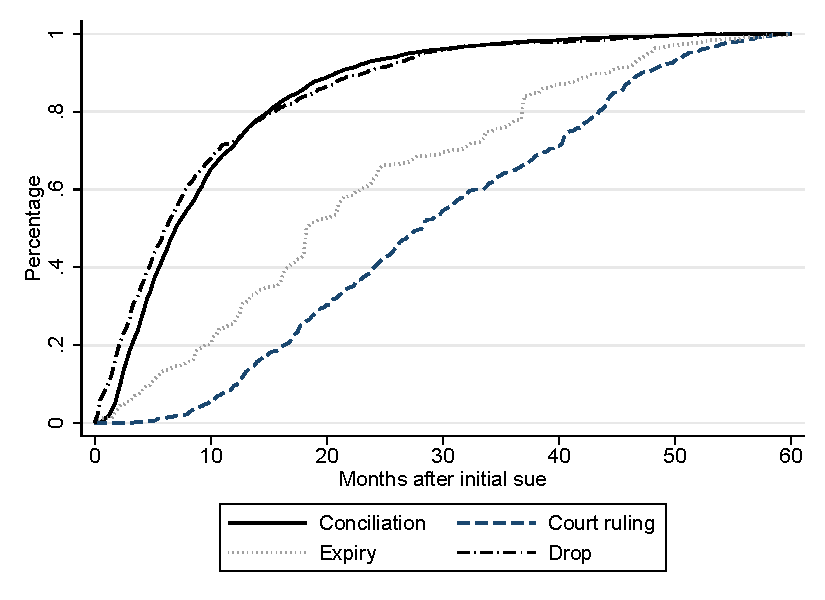
\includegraphics[width=0.6\textwidth]{caseending_overtime.pdf}
        \end{center}
\end{figure}
\end{frame}


\begin{frame}{Stylized Facts: Recovery is low}
    \begin{itemize}
        \item \textbf{Fact 2 (Awards are low):} The amount awarded is 5 to 10 times smaller than the amount asked for, and less than what the law mandates.
            
    \end{itemize}
    \begin{figure}[H]
    \label{claimsvsoutcomes}
    \begin{center}
        \includegraphics[width=0.6\textwidth]{Amountasked.tiff}
        \end{center}
    \end{figure}    
\end{frame}


\begin{frame}{Stylized Facts: Recovery is low}
    \begin{itemize}
        \item 40\% of cases filed with private lawyers have negative expected payoffs.
            
    \end{itemize}
    \begin{figure}[H]
    \label{cdf_value_claims}
    \begin{center}
        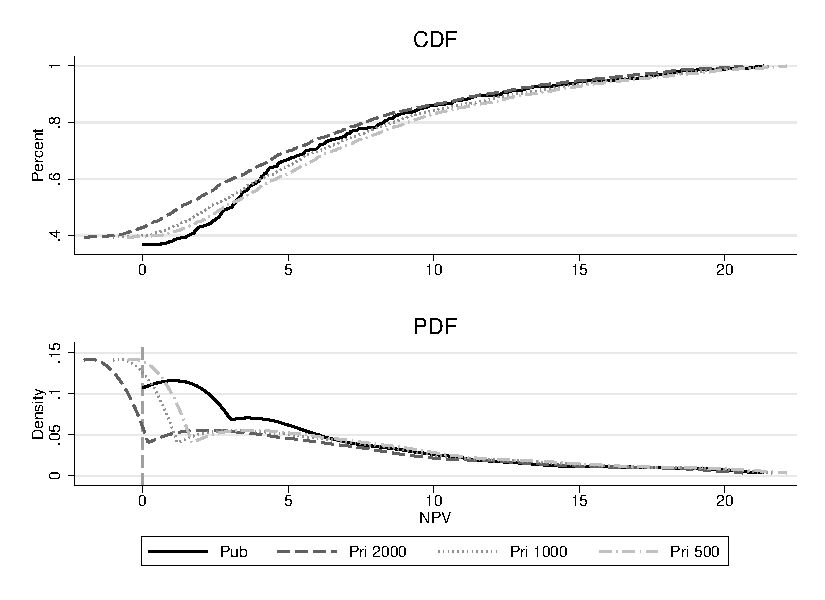
\includegraphics[width=0.6\textwidth]{cdf_pdf_value_claims.pdf}
        \end{center}
    \end{figure}    
\end{frame}


\begin{frame}{Stylized Facts: Misinformation}
    \begin{itemize}
        \item \textbf{Fact 3 (Misinformation):}
        \vspace{0.05in}
        \begin{itemize}
            \item Only 60\%  know whether they are claiming overtime in their own lawsuit. 
            \vspace{0.05in}
            \item Only one-third of workers know what the legal severance pay is.
        \end{itemize}
        
    \end{itemize}
    
       \begin{figure}[H]
    \begin{center}
        \begin{subfigure}{0.49\textwidth}
            \caption{Overtime}
            \centering
            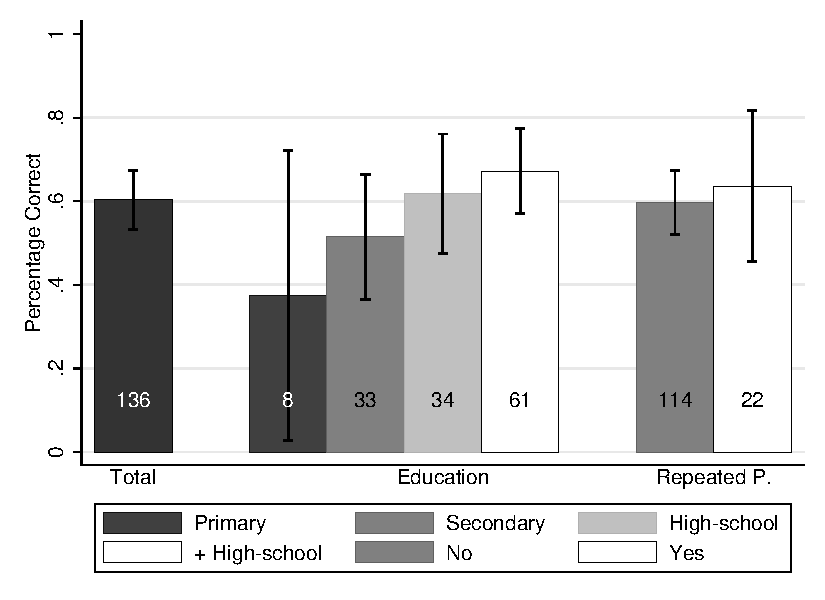
\includegraphics[width=1\textwidth]{Extra_hrs.pdf}
        \end{subfigure}
        \begin{subfigure}{0.49\textwidth}
            \caption{Severance}
                \centering
                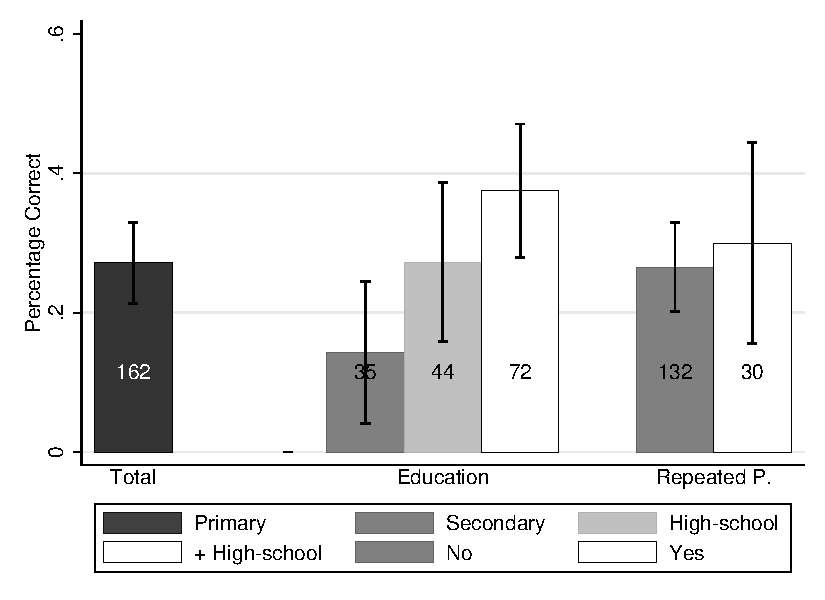
\includegraphics[width=1\textwidth]{Correctly_knows.pdf}
        \end{subfigure}
        \end{center}
\end{figure}

   
\end{frame}




\begin{frame}{Inflated expectations}
    \begin{itemize}
        \item  \textbf{Fact 4 (Overconfidence):} Plaintiffs on average think they will win 78\% of the time, while their average win rate in the data is 41\%. The sum of subjective probabilities of winning for the same cases is 1.47.
        \vspace{0.2in}
        
         \item \textbf{Fact 5 (Inflated claim and not more money awarded):} Controlling for observables, private lawyers ask for 137,592 pesos more than public lawyers, and only get 10,531 pesos more in settlements.
    \end{itemize}
  
\end{frame}



\section{Experiment and Results}

\begin{frame}{Experiment: provide information to debias parties}

    Given the environment of low information, misaligned incentives, overconfidence, and the possibility of private lawyer moral hazard...
        \vspace{0.1in}
        
    \begin{itemize}
        \item \textbf{Treatment 1: ``Calculator''.} provide (objective) statistical information that could help ''debias'' the plaintiff's expectations and lead to more settlement.
          \begin{itemize}
              \item Probability and amount won conditional on winning
              \item Unbiased prediction (out of sample tests -- good fit)
              \item Explained that is was an average for concluded cases similar to theirs.
          \end{itemize}
        \vspace{0.1in}
        \item \textbf{Treatment 2: ``Expert advice''.} Face-to-face advice from a conciliator.
        \vspace{0.1in}
        \item{\textbf{Outcomes:} settlement, \alert{expectation updating}}
         \vspace{0.1in}
        \item \textbf{Welfare:} we will not make welfare claims, but...
            \begin{itemize}
                \item The law encourages settlement.
                \item In (most?) models of asymmetric information welfare increases as the uninformed party accesses better information.
                \item We show that on average those who settle in the experiment do not receive less than their trial counterfactual.
            \end{itemize}
    \end{itemize}
\end{frame}




\begin{frame}{Experimental assignment}
\    \begin{itemize}
        \vspace{.1in}
        \item The experiment started on March 2, 2016 and ended on May 27, 2016.
        \vspace{.2in}
        \item Intervened in 1103 casefiles right before hearing.
        \vspace{0.2in}
        \item We randomized into 3 arms (control, calculator, conciliator) with equal probabilities. 
            \begin{itemize}
                \item Balance tests passed in assignment and take-up sample.
            \end{itemize}
        \vspace{0.2in}    
        \item Take up of the treatment was about 70\% in all arms. Take up exit survey 52\%. We present ITT results.
       \end{itemize} 
\end{frame}




\begin{frame}{Calculator treatment}

    \begin{figure}[H]
    \label{calc_template}
    \begin{center}
        \includegraphics[width=0.55\textwidth]{calctreat.png}
        \end{center}
\end{figure}
\end{frame}




\begin{frame}{Main Result}
    \begin{itemize}
        \item We find that \textbf{\textit{same day} conciliation increases by 4pp} for calculator and conciliator, above the 5pp for control. \alert{\textbf{Only when the worker present: 16pp effect then.}}
            \begin{itemize}
               \item We scaled it up to 5 more courts (but randomization at day level), it replicated.
                \item  Employee presence is endogenous: we tried to induce it by invitation but low take up
            \end{itemize}
        \vspace{0.05in}
        \item The effect is \textbf{persistent 5+ months later}, therefore not a ''lagged-communication'' story. 
        \vspace{0.05in}
        
    \end{itemize}
  \hskip-5.0cm
 \begin{table}
    \label{Treatment_effects}
    \tiny{\begin{tabular}{lccccccccc}
\toprule
\multicolumn{1}{|r}{} & \multicolumn{9}{c}{Months after treatment} \\
\midrule
\multicolumn{1}{r|}{} & \multicolumn{5}{c|}{Same day settlement} & \multicolumn{1}{c|}{2 months } & \multicolumn{1}{c|}{ 5 months} & \multicolumn{1}{c|}{Long run} & Same day  \\
\midrule
\midrule
\multicolumn{1}{r|}{} & \multicolumn{2}{c|}{Phase 1} & \multicolumn{2}{c|}{Phase 2} & \multicolumn{5}{c}{Phase 1/2} \\
\midrule
\multicolumn{1}{r|}{} & \multicolumn{5}{c|}{OLS}              & \multicolumn{3}{c|}{OLS} & CF OLS \\
\midrule
\midrule
      & (1)   & (2)   & (3)   & (4)   & (5)   & (6)   & (7)   & (8)   & (9) \\
Control (constant) & 0.060*** & 0.034*** & 0.11*** & 0.10*** & 0.094*** & 0.15*** & 0.39*** & 0.45*** & 0.034 \\
      & (0.013) & (0.011) & (0.030) & (0.030) & (0.026) & (0.043) & (0.039) & (0.049) & (0.043) \\
Calculator & 0.051** & 0.019 & 0.047** & 0.0077 & 0.018 & 0.0035 & -0.0069 & -0.0025 & 0.0043 \\
      & (0.022) & (0.019) & (0.021) & (0.019) & (0.014) & (0.021) & (0.024) & (0.025) & (0.015) \\
Emp present (EP) &       & 0.14*** &       & 0.14* & 0.14*** & 0.11** & 0.094* & 0.070 & 0.62*** \\
      &       & (0.050) &       & (0.072) & (0.041) & (0.046) & (0.048) & (0.050) & (0.23) \\
Calculator\#EP &       & 0.16** &       & 0.16* & 0.16*** & 0.18*** & 0.16** & 0.14** & 0.16*** \\
      &       & (0.079) &       & (0.089) & (0.056) & (0.061) & (0.064) & (0.061) & (0.055) \\
Control Function &       &       &       &       &       &       &       &       & -0.27** \\
      &       &       &       &       &       &       &       &       & (0.13) \\
      &       &       &       &       &       &       &       &       &  \\
\midrule
Observations & 716   & 716   & 1092  & 1092  & 1808  & 1808  & 1808  & 1808  & 1808 \\
R-squared & 0.0083 & 0.12  & 0.051 & 0.11  & 0.13  & 0.12  & 0.10  & 0.083 & 0.136 \\
Court dummies  & NO    & NO    & YES   & YES   & YES   & YES   & YES   & YES   & YES \\
Dep. var. Mean & \multicolumn{2}{c}{0.085} & \multicolumn{2}{c}{0.20} & 0.16  & 0.20  & 0.34  & 0.45  & 0.16 \\
Interaction var. Mean &       & 0.19  &       &       & \multicolumn{5}{c}{0.19} \\
\bottomrule
\bottomrule
\end{tabular}%

}
\end{table}
\end{frame}

\begin{frame}{Interpretation of results}
    We interpret the results as showing:
    \vspace{.1in}
    \begin{enumerate}
        \item The treatments do more than speed up settlements. (The treatment effects do not diminish over time.)
        
        
        \item \textit{Agency issues}: The treatment is effective only when the employee is present. 
        \item The treatment effect does not grow over time - no evidence the lawyer informs his client.
        \begin{itemize}
            \item The employer is (almost) never present, so we cannot say anything about agency on the defendant's side. 
        \end{itemize}
    \end{enumerate}
    \pause
    These results raise two questions:
    \begin{itemize}
        \item Why are incentives mis-aligned in spite of private lawyers receiving 30\% of amounts collected?
        \item What can we say about the welfare effects of the incremental settlements, from the perspective of the plaintiffs?
    \end{itemize}
\end{frame}

\begin{frame}{Counterfactual}

\begin{itemize}
    \item Using a matching (on observables) exercises, we are finding that the settled on amount is larger on average that what similar cases would get in trial. 
\end{itemize}

  \hskip-6.0cm\begin{table}
    \label{match_table}
    \tiny{% Table generated by Excel2LaTeX from sheet 'NN_match'
\begin{tabular}{lcccc|cc}
\toprule
\multicolumn{7}{c}{Treatment effect. Nearest-neighbor matching} \\
\midrule
\midrule
      & \multicolumn{6}{c}{Phase 1/2} \\
\midrule
\midrule
      & \multicolumn{4}{c|}{Variable matching} & \multicolumn{2}{c}{PSM} \\
\midrule
\midrule
      & (1)   & (2)   & (3)   & (4)   & (5)   & (6) \\
\midrule
ATE   & 3522* & 4853*** & 4290*** & 5736*** & 6646*** & 5835*** \\
      & (2031) & (1844) & (2047) & (1853) & (1805) & (1500) \\
\% ATE & 46    & 64    & 56    & 75    & 87    & 77 \\
Baseline mean & \multicolumn{6}{c}{7598} \\
Obs   & \multicolumn{6}{c}{307} \\
Obs HD & \multicolumn{6}{c}{415} \\
Bias adjustment & NO    & NO    & YES   & YES   & -     & - \\
Matches & [1-1] & [1-3] & [1-1] & [1-3] & [1-1] & [1-3] \\
\bottomrule
\bottomrule
\end{tabular}%
}
\end{table}
    \footnotesize
    \tiny{\textit{Notes:} 
Nearest-neighbors matching between casefiles from Phase 1/Phase 2 and Historical Data (HD) with the basic variables public lawyer, gender, at will worker, tenure, daily wage \& weekly hours, entitlement by law, and calculator prediction for court ruling amount. Counterfactual and settlement quantities are brought to present value at the time of suing with a monthly interest rate of $3.43$, with a $30\%$ cost, and an initial fee of \$2000 pesos for private lawyers. Col 3 is trimmed at top 1\%.}
\end{frame}


\begin{frame}{Debiasing?}
 \begin{table}[H]
  \resizebox{0.9\textwidth}{!}{\begin{minipage}{\textwidth}
\label{update_rel_oc}
\begin{center}
\scriptsize{% Table generated by Excel2LaTeX from sheet 'update_reg_theta_rel_oc'
\begin{tabular}{lccc}
\toprule
      & \multicolumn{3}{c}{Relative updating} \\
\midrule
\midrule
      & Employee & Emp Lawyer & Firm Lawyer \\
\midrule
      & (1)   & (2)   & (3) \\
\midrule
\midrule
Calculator & -0.45** & 0.63  & -0.48 \\
      & (0.21) & (3.92) & (0.62) \\
Constant  & -1.63** & -15.9 & 1.24* \\
      & (0.58) & (11.1) & (0.72) \\
      &       &       &  \\
\midrule
Observations & 30    & 79    & 58 \\
Basic Variable Controls  & YES   & YES   & YES \\
Other controls & YES   & YES   & YES \\
R-squared & 0.45  & 0.11  & 0.095 \\
Update (mean) & -0.18 & 2.58  & 0.65 \\
Update (SD) & 0.46  & 16.2  & 2.07 \\
\bottomrule
\bottomrule
\end{tabular}%
}
\end{center}
\end{minipage}}
\end{table}
 \footnotesize
\textit{Notes:} 
All regressions include basic variables as controls (Public lawyer, Gender, At will worker, Tenure, Daily wage \& Weekly hours) and sample is restricted to over-confident cases, i.e. where  $initialsurvey>P$. Other controls refer to repeated, player, level of anger and education level. It is important to note that scpecification is not robust to other controls.  Relative updating is computed as $\frac{exitsurvey-initialsurvey}{initialsurvey}$.
\end{frame}


\section*{Summary}

\begin{frame}{Summary: Evidence suggestive of private lawyer moral hazard}
  \begin{itemize}
  \item \alert{Context:} Lawyers much more informed than workers, hard to build lawyer reputation, incentives misaligned (fixed fee for suing).
    \vspace{0.05in}
  \item \alert{Inflation of initial claim:} Private lawyers ask for much more in initial suit, conditioning on observables. But they get much less than they ask for. 
    \vspace{0.05in}
  \item  The Calculator (and conciliator) increases settlement rates, but \alert{only when worker present}.
    \vspace{0.05in}
  \item Work in progress:
  \vspace{0.05in}
    \begin{itemize}
    \item \alert{Manipulate selection of lawyer} to test whether private lawyers indeed settle less and inflate expectations-- pay for UBER ride to public lawyers' office
      \vspace{0.05in}
    \item Measure expectations better and include conciliated cases.
      \vspace{0.05in}
    \item Model from plaintiff/firm asymmetric information?
      \vspace{0.05in} 
    \end{itemize}
\end{itemize}
\end{frame}



\begin{frame}{How this project started}{}
  \begin{itemize}
  \item {The title is preliminary... we need feedback.}
  \vspace{.1in}
  \item {We began the experiment with the conjecture that workers were overconfident about their likelihood of winning, and that this limited settlement.}
  \vspace{.1in}
  \item {We found some evidence for this, but discovered that lawyers \textit{\textbf{seem}} to play a role in that overconfidence.}
  \vspace{.1in}
  \item{The problem is that we don't have a smoking gun for the role of lawyers, since there is a (lawyer) selection problem.}
  \vspace{.1in}
  \item The issue is how to sell the paper to appeal to a general journal (if possible). Need your input on:
    \begin{itemize}
        \item \alert{\textbf{Possibility A:}} This is a paper about overconfidence and low settlement -- info provision helps
        \item \alert{\textbf{Possibility B:}} This is a paper about bargaining through agents and moral hazard.
    \end{itemize}
       \end{itemize}
\end{frame}


\begin{frame}{A framework for understanding the results}
    
    
\begin{claim}\footnote{$I_{w,f}:=\left\{x\;\;|\;\;\mathbb{E}_wU_w\leq x\leq\mathbb{E}_fU_f\right\}$}
\label{claim1}
Suppose $g_w(x)=g_l(x)=g_f(x):=g(x)$  and 
\[A_{U_w}(x)\geq A_{U_l}(x)\geq A_{U_f}(x)\quad ;\;\forall\;x\in \operatorname{supp} g \]
where $A_{U}(x)-\frac{U^{\prime\prime}(x)}{U^{\prime}(x)}$ is the Arrow-Pratt measure of risk aversion. Suppose further that $U_w^{\prime}(x)\leq U_l^{\prime}(x)\leq U_f^{\prime}(x)$ in a neighbourhood of $0$. Then $\emptyset\neq I_{l,f}\subseteq I_{w,f}$. That is, the worker is more willing to settle than her lawyer.
\end{claim}



\begin{claim}
\label{claim2}
Assume additionally that $g^o_w \succeq_{FOSD} g_w$. Then $I_{w^o,f} \subseteq I_{w,f}$. That is, overconfidence shrinks the settlement range
\end{claim}
\end{frame}


\begin{frame}{A framework for understanding the results}
\begin{claim}
\label{claim3}
Let the worker have a prior distribution $g_w$, and let the calculator be a signal with distribution $S$. Suppose further that the signal satisfies  $g_w \succeq_{FOSD} S$ and that the agent is Bayesian.\footnote{We say that the agent is Bayesian if he follows a \emph{Bayesian rule} according to definition in \textit{Shmaya \& Yariv. Foundations for Bayesian Updating.}} If we denote the posterior by $\hat{g}_w$, then $I_{w,f} \subseteq I_{\hat{w},f}$. That is, after updating the settlement range increases.
\end{claim}
\end{frame}



\begin{frame}{A framework for understanding the results}
    \begin{figure}[H]
   \caption{Illustration of claims}
   \label{figure}
\begin{center}
 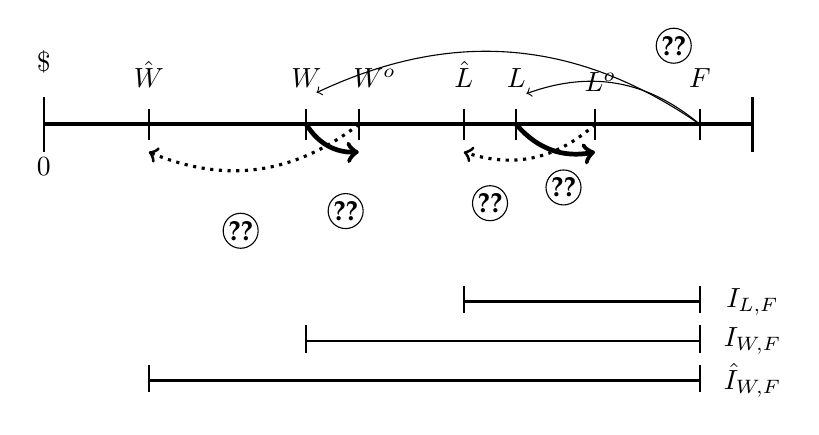
\begin{tikzpicture}
    \draw[line width=0.5mm] (0,0) -- (13.5/1.5,0) node [below] {};
    \foreach \x in {0,13.5}
    \draw[line width=0.3mm] (\x/1.5, 0.35) -- node[pos=-0.25] (point\x) {} (\x/1.5, -0.35);
    
    \foreach \x in {2, 5, 6, 8, 9, 10.5, 12.5}
    \draw[line width=0.25mm] (\x/1.5, 0.2) -- node[pos=-0.35] (point\x) {} (\x/1.5, -0.2);
    % node's content --- access them as point1...point5
    \path (point0) node [above] {$\$$};
    \path (0,-0.3) node [below] {$0$};
    \path (point2) node [above] {$\hat{W}$};
    \path (point5) node [above] {$W$};
    \path (6.3/1.5,0.35) node [above] {$W^o$};
    \path (point8) node [above] {$\hat{L}$};
    \path (point9) node [above] {$L$};
    \path (10.6/1.5,0.3) node [above] {$L^o$};
    \path (12.5/1.5,0.35) node [above] {$F$};
    
    \path (12.5/1.5,0) edge[black, bend right, ->] (point9);
    \path (12.5/1.5,0) edge[black, bend right, ->] (point5);
    \draw (12/1.5,1) node[circle,draw, inner sep=0.5pt](c1) {$\ref{claim1}$};
    
    \path (5/1.5,0) edge[black, line width=0.6mm, bend right, below, ->] (6/1.5,-0.35);
    \draw (5.75/1.5,-1.1) node[circle,draw, inner sep=0.5pt](c2) {$\ref{claim2}$};
    
    \path (9/1.5,0) edge[black, line width=0.6mm, bend right, below, ->] (10.5/1.5,-0.35);
    \draw (9.9/1.5,-0.8) node[circle,draw, inner sep=0.5pt](c2) {$\ref{claim2}$}; 
    
    \path (6/1.5,0) edge[black, line width=0.4mm, dotted, bend left, below, ->] (2/1.5,-0.35);
    \path (3.75/1.5,-1.35) node[circle,draw, inner sep=0.5pt]  {$\ref{claim3}$};

    
    \path (10.5/1.5,0) edge[black, line width=0.4mm, dotted, bend left, below, ->] (8/1.5,-0.35);
    \draw (8.5/1.5,-1.0) node[circle,draw, inner sep=0.5pt] {$\ref{claim3}$};  

    
    \draw[line width=0.3mm] (8/1.5,-2.25) -- (12.5/1.5,-2.25) node [below] {};
    \foreach \x in {8,12.5}
    \draw[line width=0.2mm] (\x/1.5, -2.05) -- node[pos=-0.25] {} (\x/1.5, -2.4);
    \path (13.5/1.5,-2.25) node  {$I_{L,F}$};
    
    \draw[line width=0.3mm] (5/1.5,-2.75) -- (12.5/1.5,-2.75) node [below] {};
    \foreach \x in {5,12.5}
    \draw[line width=0.2mm] (\x/1.5, -2.55) -- node[pos=-0.25] {} (\x/1.5, -2.9);
    \path (13.5/1.5,-2.75) node  {$I_{W,F}$}; 
    
    
    \draw[line width=0.3mm] (2/1.5,-3.25) -- (12.5/1.5,-3.25) node [below] {};
    \foreach \x in {2,12.5}
    \draw[line width=0.2mm] (\x/1.5, -3.05) -- node[pos=-0.25] {} (\x/1.5, -3.4);
    \path (13.5/1.5,-3.25) node  {$\hat{I}_{W,F}$}; 
    
  \end{tikzpicture}
 \end{center}

\end{figure} 

\end{frame}


% Placing a * after \section means it will not show in the
% outline or table of contents.


\begin{frame}[allowframebreaks]
        \frametitle{References}
    %\nocitep{*}


\printbibliography

\end{frame}

% All of the following is optional and typically not needed. 



\begin{frame}{Summary Statistics}{SS}
  \begin{table}[H]
    \label{Sum_Stats_outcomes}
    \begin{center}
       \tiny{% Table generated by Excel2LaTeX from sheet 'SS'
\begin{tabular}{lccccc}
\toprule
Variable & HD    & HD Subcourt 7 & Phase 1 & Phase 2 & Phase 3 \\
\midrule
\midrule
      & \multicolumn{5}{c}{Panel A: Outcomes} \\
\cmidrule{2-6}Win   & 0.65  & 0.69  &       &       &  \\
      & (.48) & (.46) &       &       &  \\
\multicolumn{1}{p{5.455em}}{Amount won\newline{}(thousand pesos)} & 23.92 & 20.36 &       &       &  \\
      & (56.3) & (47.49) &       &       &  \\
\multicolumn{1}{p{5.455em}}{Total asked\newline{}(thousand pesos)} & 343.06 & 301.57 & 598.32 & 644.06 &  \\
      & (655.17) & (551.15) & (1438.49) & (3860.99) &  \\
Conciliation  & 0.63  & 0.67  & 0.22  & 0.2   &  \\
      & (.48) & (.47) & (.41) & (.4)  &  \\
Losing court ruling  & 0.07  & 0.01  &       &       &  \\
      & (.25) & (.1)  &       &       &  \\
Winning court ruling & 0.02  & 0.02  &       &       &  \\
      & (.14) & (.12) &       &       &  \\
Duration (years) & 1.02  & 0.98  &       &       &  \\
      & (.96) & (.71) &       &       &  \\
\cmidrule{2-6}      & \multicolumn{5}{c}{Panel B: Basic variables} \\
\cmidrule{2-6}Public Lawyer & 0.1   & 0.15  & 0.11  & 0.06  &  \\
      & (.3)  & (.36) & (.32) & (.24) &  \\
Female & 0.48  & 0.35  & 0.42  & 0.46  & 0.45 \\
      & (.5)  & (.48) & (.49) & (.5)  & (.5) \\
At will worker & 0.07  & 0.06  & 0.18  & 0.08  &  \\
      & (.25) & (.23) & (.39) & (.27) &  \\
Tenure (years) & 4.17  & 3.72  & 4.71  & 4.33  & 3.71 \\
      & (4.99) & (4.72) & (6)   & (5.74) & (4.74) \\
Daily wage & 470   & 455   & 740   & 605   & 323 \\
      & (1100.8) & (656.22) & (1361) & (1007.75) & (634.99) \\
Weekly hours & 57.33 & 57.36 & 57.39 & 56.15 & 52.88 \\
      & (15.47) & (15.57) & (16.87) & (13.38) & (15.52) \\
      &       &       &       &       &  \\
\midrule
Observations & 5005  & 857   & 599   & 1087  & 1929 \\
\bottomrule
\bottomrule
\end{tabular}%
}
    \end{center}
\end{table}
\end{frame}


\begin{frame}{Summary Statistics}{SS}
\begin{table}[H]
    \caption{Settlements against duration - Historical Data}
    \label{settlement_time}
    \begin{center}
    \tiny{% Table generated by Excel2LaTeX from sheet 'settlementq_time'
\begin{tabular}{lcccccc}
\toprule
      & \multicolumn{2}{c}{Settlement amount} & \multicolumn{2}{c}{Settlement amt discounted} & \multicolumn{2}{c}{Calculator prediction} \\
\midrule
\midrule
      & (1)   & (2)   & (3)   & (4)   & (5)   & (6) \\
\midrule
\midrule
Months  & 1202.9*** &       & -166.3** &       & 180.0*** &  \\
      & (166.8) &       & (70.37) &       & (30.82) &  \\
2 Quintil &       & 4052.7** &       & 1754.3 &       & 1576.3*** \\
      &       & (1859.3) &       & (1676.1) &       & (460.2) \\
3 Quintil &       & 1622.4 &       & -1767.8 &       & 1451.0** \\
      &       & (2015.3) &       & (1705.6) &       & (565.7) \\
4 Quintil &       & 8663.2*** &       & 44.58 &       & 3029.1*** \\
      &       & (2348.7) &       & (1808.5) &       & (595.2) \\
5 Quintil &       & 21982.6*** &       & -3474.0* &       & 3990.9*** \\
      &       & (3299.9) &       & (1882.0) &       & (718.8) \\
Constant  & 10907.8*** & 15396.9*** & 15841.8*** & 14649.2*** & 9544.0*** & 9331.9*** \\
      & (4229.2) & (4326.9) & (2953.9) & (3018.0) & (1031.9) & (1076.7) \\
      &       &       &       &       &       &  \\
\midrule
Observations  & 3080  & 3080  & 3080  & 3080  & 3081  & 3081 \\
R-squared & 0.24  & 0.23  & 0.22  & 0.22  & 0.66  & 0.65 \\
BVC   & YES   & YES   & YES   & YES   & YES   & YES \\
\bottomrule
\bottomrule
\end{tabular}%
}
    \end{center}
     \scriptsize
    \textit{Notes:} 
    This table focuses on the sample of cases from the historical data (HD) that settled at any point in time (3080 cases out of 5005). Each column is a different regression. All regressions control for the basic variables of the case (BVC) which are described in Panel B of Table 1. Columns 1 and 2 have as a dependent variable the settlement amount in pesos the worker actually got in the settlement. Column 1 regresses this amount on a counter for the number of months that elapsed from the initial filing until the settlement. Column 2 breaks this elapsed time in quintiles dummies. Columns 3 and 4 discount the peso amount at a 3.43 monthly rate. This rate was calculated by matching our sample to that of the MxFls survey and obtaining the elicited time discount rate for similar individuals (using gender, age, education, daily wage, and weekly hours), and taking the median. Columns 5 and 6 use the prediction from our ``calculator'', that is, the amount they would get on average given the initial case characteristics, with no discounting.
    %\textit{Do file: } \texttt{settlementq\_time.do}
\end{table}
\end{frame}




\begin{frame}{Expectations for different parties}
\begin{table}[H]
    \label{prediction_cases}
    \begin{center}
       \scriptsize{% Table generated by Excel2LaTeX from sheet 'prediction_cases_pooled'
\begin{tabular}{lcccc}
\toprule
      & \multicolumn{2}{c}{Expectation} & \multicolumn{2}{c}{Relative OC} \\
\midrule
\midrule
      & Probability & Amount & Probability & Amount \\
\midrule
      & (1)   & (2)   & (3)   & (4) \\
\midrule
\midrule
Employee's Lawyer & 4.52  & 5902.2 & 0.22  & -0.097 \\
      & (3.46) & (12555.8) & (0.14) & (0.53) \\
Firm's Lawyer & -27.4*** & -27573.0** & -0.96*** & -0.38 \\
      & (3.34) & (12083.0) & (0.13) & (0.50) \\
Constant & 75.0*** & 74788.7*** & 1.64*** & 0.73* \\
      & (2.86) & (10219.5) & (0.11) & (0.43) \\
      &       &       &       &  \\
\midrule
Observations & 2214  & 1859  & 1952  & 1632 \\
File Fixed Effects & YES   & YES   & YES   & YES \\
R-squared & 0.83  & 0.89  & 0.96  & 0.89 \\
p-value:Emp Law & 0     & 0     & 0     & 0 \\
p-value:Firm Law & 0     & 0     & 0     & 0.1 \\
\bottomrule
\bottomrule
\end{tabular}%
}
    \end{center}
\end{table}
    \footnotesize    
    \textit{Notes:} 
     The table regresses measures of expectation elicited in the baseline survey on dummies of who is the respondent of the survey. For some cases we could elicit the expectation of more than one party (employee, employee's lawyer, firm's lawyer). The omitted variable is the employee dummy, so the interpretation of the employee's lawyer and firm's lawyer coefficients are relative to the employee who is captured in the constant. It combines two phases in one singled pooled dataset. Each column represents a different regression. The first column use elicited probability of winning as a dependent variable. The exact question is: \textit{``How likely is it that you will win the lawsuit if it ends in a court judgment?''}. The second column use the peso amount (undiscounted) that they expect to recover conditional on winning. The exact wording of the survey question is: \textit{``in case you win the lawsuit, what amount are you most likely to win?''}.  All columns include casefile fixed effects, avoiding the comparison across casefiles. The bottom of the table present the p-values of two null hypothesis:  $\alpha + \beta_1=0$, and $\alpha + \beta_2=0$, telling us whether the employee's laywer, or the firm or firm's lawyer are accurate in their predictions. Last 2 columns use a measure of ``overconfidence'', which compares the subjective expectation vs the personalized calculator prediction. Relative OC is computed as $\frac{expectation-prediction}{prediction}$, where expectation refers to the expectation measured in the baseline survey.
\end{frame}


\begin{frame}{The Effect of Treatment on the Settlement Amounts}
\begin{table}[H]
    \label{SS_OC}
    \begin{center}
       \scriptsize{\input{../paper/Tables/settlement_conciliator.tex}}
    \end{center}
\end{table}
\footnotesize
\textit{Notes:}
This table focuses on our workers that conciliated within our experimental samples in the same day as treatment. It regresses the (undiscounted) settlement amount against treatment dummies. When the worker is served by a private lawyer we subtract \$2000 from the initial fee, as well as 30\% of the settlement amount. These numbers are the median responses from our baseline survey on how the private lawyers are paid. Each column is a different regression. Column 1 for instance shows that 173 settled on the same day as the treatment. Column 2 controls for the BVC's (observations differ since there are some missing values in the basic variable controls), while Column 3 also includes the calculator prediction (``counter factual-court ruling amount'') as well as the entitlement by law for unfair dismissal assuming the worker wins the case.
\end{frame}



\begin{frame}{Baseline Expectations}
\begin{table}[H]
    \label{Table_expectations}
    \begin{center}
       \scriptsize{\input{../paper/Tables/SS_A.tex}}
    \end{center}
\end{table}
    \footnotesize    
    \textit{Notes:} 
    Summary statistics of parties' beliefs. We show mean and standard deviation for the whole sample, \& dividing by type of employee's lawyer.
\end{frame}



\begin{frame}{Compliance rate}
 \begin{table}[H]
  \resizebox{0.9\textwidth}{!}{\begin{minipage}{\textwidth}
\label{Table_compliance}
\begin{center}
\scriptsize{% Table generated by Excel2LaTeX from sheet 'Compliance'
\begin{tabular}{lrcccccccccccc}
\toprule
\multicolumn{1}{c}{Group} & \multicolumn{1}{c}{N} & \multicolumn{4}{c}{Compliance with treatment} & \multicolumn{4}{c}{Compliance with baseline survey} & \multicolumn{4}{c}{Compliance with exit survey} \\
\midrule
\midrule
      &       & Plaintiff & Defendant & Both  & Any   & Plaintiff & Defendant & Both  & Any   & Plaintiff & Defendant & Both  & Any \\
\midrule
Control & 321   & -     & -     & -     & -     & 50.78 & 35.51 & 8.72  & 77.57 & 39.88 & 24.3  & 5.61  & 58.57 \\
Calculator & 315   & 77.65 & 73.03 & 75.81 & 79.72 & 48.25 & 33.65 & 12.38 & 69.52 & 38.63 & 25.86 & 9.66  & 54.83 \\
\bottomrule
\end{tabular}%
}
\end{center}
\end{minipage}}
\end{table}
 \footnotesize
\textit{Notes:} 
The number of cases assigned to the 3 different groups is very similar, and is close to 7 per day on average. The compliance with treatment rate is similar for both treatments and in the range of 75\%.
\end{frame}


\begin{frame}{Employee presence}
\begin{table}[H]
    \label{pactor_reg}
    \begin{center}
    \scriptsize{% Table generated by Excel2LaTeX from sheet 'pactor_reg'
\begin{tabular}{lccc}
\toprule
      & \multicolumn{3}{c}{Employee Present} \\
\midrule
\midrule
      & Phase 1 & Phase 2 & Phase 1/2 \\
\midrule
\midrule
      & (1)   & (2)   & (3) \\
\midrule
\midrule
Female & -0.066* & 0.000 & -0.023 \\
      & (0.035) & (0.023) & (0.019) \\
Public Lawyer & 0.317*** & 0.508*** & 0.416*** \\
      & (0.066) & (0.059) & (0.045) \\
At will worker & -0.063 & 0.013 & -0.016 \\
      & (0.049) & (0.042) & (0.032) \\
Tenure (years) & 0.004 & 0.005** & 0.005*** \\
      & (0.003) & (0.002) & (0.002) \\
Daily wage & -0.000 & -0.000 & -0.000 \\
      & (0.000) & (0.000) & (0.000) \\
Weeky hours & -0.002** & -0.003*** & -0.003*** \\
      & (0.001) & (0.001) & (0.001) \\
Age   &       & -0.001 &  \\
      &       & (0.003) &  \\
Constant & 0.313*** & 0.303*** & 0.298*** \\
      & (0.062) & (0.066) & (0.045) \\
      &       &       &  \\
\midrule
Observations & 520   & 1026  & 1546 \\
R-squared & 0.090 & 0.124 & 0.105 \\
DepVarMean & 0.208 & 0.183 & 0.191 \\
p-value & 0.000 & 0.000 & 0.000 \\
p-value w/o PL & 0.014 & 0.001 & 0.000 \\
\bottomrule
\bottomrule
\end{tabular}%
}
    \end{center}
    \scriptsize
    \textit{Notes:} OLS of employee presence against basic variable controls as predictors. Last two rows shows the p-value testing the quality of all basic variables ( \& without public lawyer) respectively.
\end{table}
\end{frame}

\end{document}


